\section{Unused cocores, a genus budget, and initial admissibility}
\label{sec:unused-handles}

The maintained initial handle operator removes geometric two/three-handle
pairs, removes geometric one/two-handle pairs, and tests exposed cocores by
transporting a dual integral cocycle to the original boundary.  Its output
explicitly stops short of an admissibility assertion: an unused one-handle
has two characteristic zero-handles of index $-4$.  The final paragraph of
the maintained \texttt{source\_handles.tex} identifies unused bridges and
their ball sides as a next operation.  We resolve that initial, empty-pattern
operation simultaneously for all unused handles.  No later boundary pattern
is discarded.

The topological ingredients---disc cutting, irreducibility, and boundary
connected sum---are classical.  The contribution here is an exact budget
for their source-handle quotient, an authenticated initial compiler, a
smaller certificate on a specified family, and a faster independent replay
of the supplied cancellation trace.  This is an explicit specialization of
Lackenby's admissibility procedure, not a claim to invent admissibility or
to complete the general patterned hierarchy.

\subsection{The geometric quotient}

Let $M$ be a compact connected orientable three-manifold with nonempty
boundary.  Consider a finite handle presentation containing zero-, one-,
and two-handles, with all three-handles already removed.  For a one-handle
$e$, let $d(e)$ be the total number of its intersections with all two-handle
attaching curves, counted as geometric occurrences.  Oppositely oriented
passages both contribute one.  Call $e$ \emph{unused} if $d(e)=0$ and
\emph{used} otherwise.

The graph of zero- and one-handles has one vertex for each zero-handle
and one edge for each one-handle, with loops and parallel edges retained.
Delete its unused edges.  For each resulting connected vertex block, take
the zero-handles in that block, its used one-handles, and all two-handles
attached there.  Write the resulting connected three-manifolds, after
rounding corners, as $K_1,\ldots,K_r$.  Define $Q$ to have these $r$ pieces
as vertices and the unused one-handles as edges.  Thus an edge of $Q$ retains
its source one-handle identifier and its two oriented endpoint occurrences.
Put
\[
  \beta=|E(Q)|-|V(Q)|+1.
\]

\begin{lemma}[Exact unused-cocore decomposition]
\label{lem:unused-decomposition}
Every two-handle belongs to exactly one $K_i$.  The graph $Q$ is connected,
and cutting $M$ simultaneously along the cocores of all unused one-handles
gives precisely the pieces $K_i$.  In particular,
\begin{equation}
 \chi(M)=\sum_{i=1}^r\chi(K_i)-|E(Q)|.
 \label{eq:unused-euler}
\end{equation}
Moreover, with arbitrary choices of connecting paths,
\begin{equation}
 \pi_1(M)\cong
 \left(\mathop{\ast}_{i=1}^r\pi_1(K_i)\right)\ast F_\beta.
 \label{eq:unused-free-product}
\end{equation}
\end{lemma}

\begin{proof}
An attaching circle cannot pass through an unused handle.  Its successive
zero-handle passages are therefore connected by used edges and belong to
one block.  This gives a well-defined, complete assignment of two-handles.
The cocore of an unused one-handle is a properly embedded disc because its
boundary misses all two-handle attaching regions.  The chosen cocores are
disjoint.  Cutting each product $D^2\times I$ across $D^2\times\{1/2\}$
and absorbing the two half-products into its endpoint zero-handles removes
the corresponding graph edge and no used handle.  Thus the connected
pieces are exactly those defined above.

The original manifold is connected and adding handles of index two does
not connect graph components, so $Q$ is connected.  Reattaching one unused
one-handle decreases Euler characteristic by one, which proves
\eqref{eq:unused-euler}.  First attach a spanning tree of $Q$.  Each edge
joins two components along discs, and van Kampen gives their free product.
Each of the remaining $\beta$ one-handles adds one free generator and no
relation.  This proves \eqref{eq:unused-free-product}.
\end{proof}

The quotient uses actual attaching occurrences.  Replacing an attaching
word by its abelianized coefficient row before deciding whether a handle
is unused invalidates the lemma.  In particular, exponent sum zero is not
geometric disjointness.

\subsection{The genus budget in a torus source}

Lemma~\ref{lem:disc-euler} shows that, under authenticated irreducibility,
the $K_i$ are irreducible, Euler characteristic one identifies precisely
the ball pieces, and every nonball piece has nonpositive Euler
characteristic.  Let $\mathcal N$ index the nonball pieces.
Theorem~\ref{thm:genus-budget} specializes to
\begin{equation}
 g=\beta+\sum_{i\in\mathcal N}\bigl(1-\chi(K_i)\bigr),
 \qquad \beta+|\mathcal N|\leq g,
 \label{eq:unused-genus-budget}
\end{equation}
when the source boundary is connected of genus $g$.
The number of ball pieces is absent from this identity.  Its torus case
has a particularly strong consequence for the initial source operator.

\begin{corollary}[Torus dichotomy]
\label{cor:unused-torus}
For an irreducible $M$ with one torus boundary, exactly one of the following
numerical cases occurs.
\begin{enumerate}
 \item $\beta=1$ and every $K_i$ is a ball.  Then $M$ is a solid torus.
 \item $\beta=0$, exactly one $K_i$ has Euler characteristic zero, and all
 other pieces are balls.  The graph $Q$ is a tree, the exceptional piece
 has one torus boundary, and it is homeomorphic to $M$.
\end{enumerate}
The second case is compatible with both trivial and nontrivial knots.
\end{corollary}

\begin{proof}
Every term of \eqref{eq:unused-genus-budget} is a nonnegative integer,
and the total is one.  If $\beta=1$, there is no nonball piece.  Attach a
spanning tree of $Q$ to the balls; the result is a ball.  Its single remaining
one-handle makes a solid torus.

Otherwise $\beta=0$ and there is exactly one nonball piece, whose Euler
characteristic is zero.  A connected graph of cycle rank zero is a tree.
Each reattached tree edge joins different manifold components and hence
joins two different boundary components.  If $b_i$ is the number of boundary
components of $K_i$, then
\[
 1=\sum_i b_i-(r-1).
\]
Each $b_i\geq1$, so every $b_i=1$.  The nonball piece therefore has a
connected boundary of genus one.  A boundary connected sum with a ball
does not change a manifold's homeomorphism type.  Absorbing the ball pieces
along the tree proves the claim.
\end{proof}

\subsection{The complete initial empty-pattern compiler}

For a triangulated source, the maintained construction has $O(t)$ handles
and $O(t)$ attaching occurrences, where $t$ is the number of tetrahedra.
The first queue removes a two-handle meeting exactly one surviving
three-handle, with endpoint multiplicity retained.  Every source interior
vertex is connected to the boundary in the one-skeleton, so this phase
removes all three-handles.  The second queue removes a one-handle meeting
exactly one two-handle in exactly one disc, counted across \emph{all}
surviving two-handles.  No surviving two-handle passes through the cancelled
one-handle, so no implicit handle slides or relator substitutions are used.
These are precisely the geometric prerequisites of the maintained
source-handle cancellation trace.

At the fixed point, every surviving one-handle has degree zero or at least
two.  Applying Corollary~\ref{cor:unused-torus} gives the following result.

\begin{lemma}[The local tetrahedral characteristic graph]
\label{lem:unused-k4}
After the stated deletion-only reductions and removal of unused handles,
the characteristic graph in each zero-handle of the retained torus core is
a nonempty connected simple subgraph of $K_4$.  Its regular neighbourhood
is the characteristic surface, and every complementary region in the
zero-handle boundary is a disc.  Up to tetrahedral symmetries, its four
possible graph types are $C_3$, $C_4$, $K_4-e$, and $K_4$.  Every
characteristic zero-handle has index zero or two; the total indices in
these four local types are respectively zero, zero, four, and eight.
\end{lemma}
\begin{proof}
The vertices of the local characteristic graph are the surviving formal
facet ports of the source tetrahedron.  There are at most four.  A surviving
characteristic strip corresponds to an original local tetrahedral edge
and joins its two distinct incident facets.  There is at most one such
local edge for each unordered pair of facets.  Thus the graph is simple,
even if different local vertices or strips have the same \emph{global}
handle identifier.  The recorded reductions only delete whole handles;
they do not identify local ports or insert new characteristic strips.

The degree at either local end of a surviving one-handle $e$ is exactly
its geometric attaching-occurrence count $d(e)$.  This count is at least
two after the degree-one cancellations and unused-handle removal.  Every
nonempty connected component of a simple graph of minimum degree at least
two has at least three vertices.  Two such components cannot fit on at
most four vertices.  Hence the local graph is connected whenever nonempty.

A zero-handle in the retained used-edge component has a used port unless
it is the sole zero-handle of an isolated component.  In that exceptional
case no source two-handle can attach there without a one-handle passage,
and its component is a ball of Euler characteristic one, so it is not
retained.  Thus every retained local graph is nonempty.  The regular
neighbourhood of a connected graph embedded in a sphere is a connected
planar surface, and all its complementary components are discs.

For completeness, three local vertices force the triangle $C_3$.  With
four vertices, every degree is two or three.  The graph has four, five,
or six edges.  The four-edge case is $C_4$, since every degree is two;
the five-edge case deletes exactly one edge from $K_4$; and the six-edge
case is $K_4$.  These are the four types listed, with their embeddings
in the tetrahedral sphere inherited from the source.  A local port of
degree $d$ has index $-4+2d$, which proves the stated index bounds and
totals.
\end{proof}

\begin{figure}[htbp]
\centering
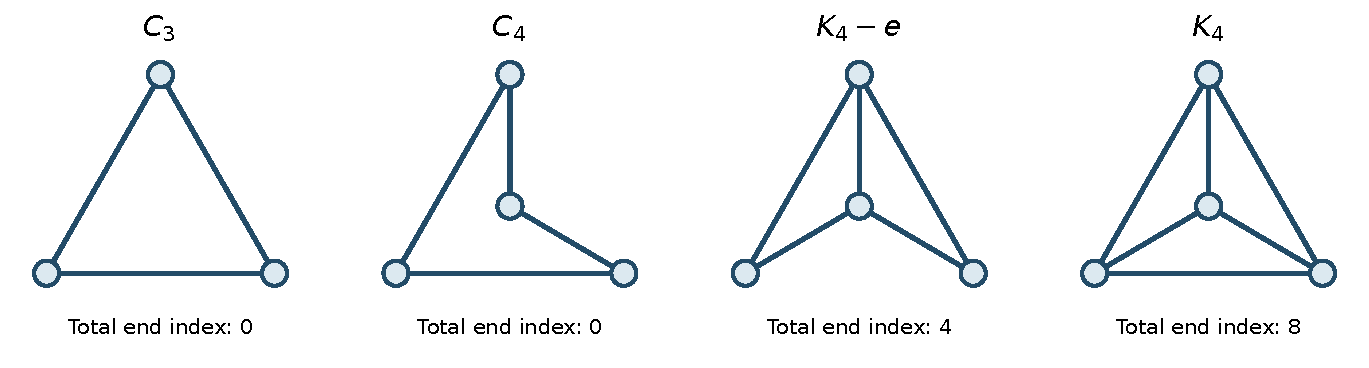
\includegraphics[width=\linewidth]{figures/local_characteristic_graphs.pdf}
\caption{The four possible nonempty local characteristic graphs in the
retained initial core.  Nodes are formal local face-port discs; edges are
surviving two-handle strips.  Every end has index zero or two.  The drawing
is a combinatorial schematic; the actual source embedding is retained in
the certificate.}
\label{fig:local-characteristic-graphs}
\end{figure}

\begin{theorem}[Initial admissibility with authenticated irreducibility]
\label{thm:unused-initial-compiler}
Given a finite triangulation of a compact connected orientable irreducible
three-manifold with one torus boundary and empty boundary pattern, the
incidence cancellations and unused-cocore quotient give, in polynomial
encoded time, either
\begin{enumerate}
 \item a solid-torus certificate from the first case of
 Corollary~\ref{cor:unused-torus}; or
 \item an inherited handle presentation, homeomorphic to the source,
 that is admissible for the empty pattern.
\end{enumerate}
The second output consists of the handles in the unique Euler-zero piece;
the source charts and cancellation trace retain their provenance.  No
normal surface search or boundary-period transport is required.
\end{theorem}

\begin{proof}
Termination and polynomial cost of the cancellation queues follow because
each move removes a handle pair and each attaching occurrence is removed
at most once.  The quotient and Euler counts are finite graph operations.
In the cycle case the preceding corollary gives the solid torus.

In the tree case cut all unused cocores and retain the unique Euler-zero
piece.  The other pieces are balls, and the corollary gives a homeomorphism
with the original manifold.  Every one-handle of the retained presentation
is used and hence has $d(e)\geq2$.  Each of its characteristic zero-handle
ends has index
\[
   -4+2d(e)\geq0.
\]
An index-zero end is disjoint from the pattern, because the pattern is empty.
For the second condition, Lemma~\ref{lem:unused-k4} shows that every
complementary region of the characteristic surface in a zero-handle
boundary is a disc.  A simple closed curve disjoint from the characteristic
surface therefore bounds a disc in that same complement, and the disc
meets the empty pattern in the empty set.  This proves the stronger
complement-disc condition, as well as the printed admissibility condition;
we do not rely on the weaker observation that an arbitrary sphere curve
bounds a disc that might contain characteristic handles.  Both required
conditions therefore hold.
\end{proof}

The retained core is a handle subpresentation, not a fresh triangulation.
It includes inherited source identifiers, its assigned two-handles, and
the geometric reduction trace.  This suffices to authenticate its unmarked
homeomorphism type and initial admissibility.  It does not provide an
explicit parametrization of every discarded ball, a transport map for an
arbitrary later pattern, or a normal-coordinate adapter on a retriangulated
core.  Those remain implementation tasks.

For an input knot diagram, the implementation's wrapper independently checks
that the supplied triangulation is the canonical exterior of that exact
classical one-component diagram.  A knot exterior in the three-sphere is
irreducible: a sphere disjoint from the connected knot bounds a ball on the
side not containing the knot.  Thus the wrapper authenticates the theorem's
hypothesis.  It returns \texttt{UNKNOT} in the cycle case and
\texttt{ADMISSIBLE\_CORE} in the tree case.  The latter is an intermediate
result, never a knottedness certificate.

\subsection{Why the irreducibility gate cannot be replaced by a flag}

The delivered exact controls \texttt{solid\_torus\_sum\_rp3} and
\texttt{solid\_torus\_sum\_s2xs1}, copied from the pinned source corpus,
are reducible manifolds with torus boundary.  Both produce $\beta=1$ with
Euler characteristic one for every cut piece.  An independent Regina
check finds that neither is a solid torus.  In particular, the quotient
and the Euler data alone do not distinguish the ball pieces from punctured
closed summands.

This has a direct classical model.  Let $N$ be a closed orientable
three-manifold other than the sphere, remove a ball, and take the boundary
connected sum of the resulting punctured manifold with a solid torus.
The result is the connected sum of the solid torus and $N$.  Cutting a
meridian cocore leaves a piece with Euler characteristic one, but the
punctured $N$ remains.  If $N=\mathbb{RP}^3$, its fundamental group already
precludes a ball.  If $N=S^2\times S^1$, the additional infinite-cyclic
free factor does the same.

The generic \texttt{verify\_unused\_handle\_certificate} therefore
authenticates only the geometric decomposition and its numerical case.
It never authorizes an irreducibility assertion from a caller's Boolean.
The diagram wrapper verifies exterior provenance first.  Mutating a valid
diagram certificate to substitute either reducible source is rejected.

\subsection{Linear replay of geometric cancellation traces}

The maintained independent cancellation checker reconstructs source cells
separately from the producer.  For each proposed one/two-handle cancellation
it scans every surviving two-handle attaching cycle to confirm that the
selected one-handle occurs once in total.  This is sound but can repeatedly
scan the same surviving rows.

\begin{proposition}[Occurrence-count replay]
\label{prop:unused-linear-replay}
After independently reconstructing the geometric attaching rows, a supplied
cancellation trace with $h$ handles and $L$ attaching occurrences can be
checked using $O(h+L)$ combinatorial incidence updates, excluding ordered
output construction and source reconstruction.  Its acceptance condition
for each one/two cancellation is identical to the full-scan condition.
\end{proposition}

\begin{proof}
Let $m_{ef}$ be the nonnegative number of occurrences of one-handle $f$
in the attaching circle of two-handle $e$.  Initialize
$d_f=\sum_{e\text{ alive}}m_{ef}$.  Deleting $e$ subtracts $m_{ef}$ from
$d_f$ for every nonzero entry of that row.  At a proposed cancellation
of $f$ with $e$, require both to be alive and require
\[
   d_f=1,\qquad m_{ef}=1.
\]
Since all multiplicities are nonnegative, these conditions say exactly
that $e$ supplies the unique geometric occurrence of $f$ among all alive
two-handles.  Signed cancellation plays no role.  The two/three-handle
condition is checked separately using the surviving endpoint occurrences,
and its deleted row is charged in exactly the same way.

Each row is deleted at most once.  Its incidence entries are visited once
at initialization and once at deletion.  The handle-state tests and final
counts use linear additional work.  An independently recomputed final
degree table can be checked in one further pass without changing the bound.
\end{proof}

The prototype uses union by size and path compression for the producer's
quotient, followed by canonical component numbering.  The verifier uses
breadth-first search on separately reconstructed raw source cells, without
calling the producer, its union-find routine, or its scheduler.  It also checks the local facet ports and source-edge strips in
Lemma~\ref{lem:unused-k4}, including their geometric degrees and local
connectedness.  The two paths share immutable input formats and elementary arithmetic; the source
geometry constructions are the established distinct maintained paths.

All source identifiers, degrees, and component sizes have $O(\log(t+1))$
bits.  The incidence and quotient certificates contain $O(t)$ records and
therefore occupy $O(t\log(t+1))$ bits.  Original source validation,
fingerprinting, and raw-cell reconstruction remain additional polynomial
costs.  The linear incidence theorem does not assert that the entire Python
source-validation stack has linear bit complexity.

\subsection{A proved certificate-size separation on Fibonacci layered tori}
\label{subsec:unused-fibonacci}

The standard layered-solid-torus fixture makes the eliminated boundary
arithmetic explicit.  Number its tetrahedra $0,\ldots,t-1$.  For
$i<t-1$, face zero of tetrahedron $i$ is paired to face two of $i+1$ by
the vertex permutation $(2,1,3,0)$, and face one is paired to face three
of $i+1$ by $(0,3,1,2)$.  In the last tetrahedron, face zero is paired to
face one by $(1,2,3,0)$.  Reverse pairings are the inverse permutations;
faces two and three of tetrahedron zero remain boundary.  This is the
maintained Fibonacci layered-solid-torus family, not a newly proposed
topological construction.

For $0\leq i\leq t-2$, write $a_i,b_i$ for the dual one-handles of face
zero and face one of tetrahedron $i$, and write $c$ for the final self-paired
handle.  Their native identifiers are $2i,2i+1,2t-2$, respectively.
Following the interior-edge links through the displayed face permutations
gives the attaching words
\begin{align}
 r_i&=b_i a_{i+1}a_{i+2}b_{i+2}^{-1}b_{i+1}^{-1}a_i^{-1}
     &&(0\leq i\leq t-4),\
 r_{t-3}&=b_{t-3}a_{t-2}c\,b_{t-2}^{-1}a_{t-3}^{-1},\
 r_{t-2}&=b_{t-2}c^2a_{t-2}^{-1}.
 \label{eq:unused-layered-relators}
\end{align}
The penultimate line is present for $t\geq3$, the last for $t\geq2$;
the case $t=1$ has only $c$ and no two-handle.  The first line is the
repeating six-sector link.  The final two lines are its five-sector and
four-sector closures at the self-paired end.  Here is an explicit check of
the three local types.  Write $(j,uv;p,q)$ for the sector at edge $uv$ in
tetrahedron $j$, entering through facet $p$ and leaving through facet $q$.
For $0\leq i\leq t-4$ the successive sectors are
\[
\begin{aligned}
 &(i,23;0,1)\longrightarrow(i+1,12;3,0)
     \longrightarrow(i+2,13;2,0)\\
 &\hspace{6mm}\longrightarrow(i+3,01;2,3)
     \longrightarrow(i+2,02;1,3)
     \longrightarrow(i+1,03;1,2).
\end{aligned}
\]
The last exit returns to the first entry.  At $i=t-3$, the self-pairing
replaces the middle step through tetrahedron $i+3$ by a direct passage
from $(i+2,13;2,0)$ to $(i+2,02;1,3)$, giving the five-sector word.
At $i=t-2$, the four sectors are
\[
 (i,23;0,1)\longrightarrow(i+1,12;3,0)
 \longrightarrow(i+1,23;1,0)
 \longrightarrow(i+1,03;1,2).
\]
Reading the exiting facet pairings gives exactly
\eqref{eq:unused-layered-relators}, including two successive positive
crossings of $c$ in the last case.  The calculation uses only the displayed
face permutations, so it proves the words for every $t$.

\begin{proposition}[Fibonacci transport and certificate separation]
\label{prop:unused-fibonacci-separation}
For this family, the maintained queue cancels $(a_i,r_i)$ in the order
$i=0,\ldots,t-2$.  Its remaining one-handles are $b_0,\ldots,b_{t-2},c$.
The native transported cocycle for the surviving cocore $c$ has
\begin{equation}
  x(b_i)=0,\qquad x(c)=1,\qquad x(a_i)=F_{t-i+1}.
  \label{eq:unused-fibonacci-values}
\end{equation}
Consequently, the native explicit dual-value list alone occupies
$\Theta(t^2)$ binary bits.  The new source incidence/component certificate
occupies $O(t\log(t+1))$ bits and contains no transported cocycle.
\end{proposition}

\begin{proof}
Initially $a_0$ occurs exactly once.  After rows $r_0,\ldots,r_{i-1}$
are removed, $a_i$ occurs exactly once in $r_i$.  The native queue places
$a_i$ before $b_i$: in the row whose removal first makes them unique,
the occurrence of $a_i$ precedes that of $b_i$.  Once $a_i$ is cancelled,
the pending $b_i$ has degree zero and is skipped.  Future $a_j$ have more
than one occurrence until this step, and $c$ retains its double occurrence
in the final row.  This proves the stated cancellation order and remainder.

The remaining $b_i$ form a tree joining the $t$ zero-handles, while $c$
is its single additional loop.  The surviving-cocore assignment sets all
$b_i$ to zero and $c$ to one.  Reading the final two equations in
\eqref{eq:unused-layered-relators} gives
\[
 x(a_{t-2})=2,\qquad x(a_{t-3})=3.
\]
Every preceding row gives
\[
 x(a_i)=x(a_{i+1})+x(a_{i+2}).
\]
Uniqueness of reverse substitution proves \eqref{eq:unused-fibonacci-values},
including the two small end cases.

The $t$ nonzero values are $F_2,F_3,\ldots,F_{t+1}$.  The recurrence gives
$F_{j+2}\geq2F_j$ and $F_j\leq2^{j-1}$, so
$\log_2 F_j=\Theta(j)$.  Summing their individual bit lengths proves the
quadratic bound.  In the new quotient every $K_i$ is just one zero-handle,
$Q$ has $t$ edges and $t$ vertices, and the trace has $t-1$ cancellations.
All identifiers are bounded by a constant multiple of $t$, proving the
new upper bound.
\end{proof}

This is a comparison with the maintained explicit coordinate-list
certificate, not a lower bound on every possible cocycle encoding.  A
recurrence-based encoding could also compress those Fibonacci integers.
The new certificate avoids constructing and checking them at all because
the authenticated geometric situation supplies a different proof.
For general input diagrams the second branch of
Theorem~\ref{thm:unused-initial-compiler} may remain, so this size separation
does not prove completeness of a polynomial unknot-recognition method.

\subsection{Finite verification and performance scope}

The delivered tests replay all 48 supplied source triangulations and compare
the new cancellation sequence, remaining handle sets, summary, and source
fingerprint with the maintained implementation.  The same incidence-only
certificates also pass the unchanged maintained cancellation verifier.
Additional checks cover 48 independent local/global relabellings, canonical
diagram exteriors, forged component lists and cycle ranks, Boolean labels,
wrong diagram provenance, caps, cooperative interruption, and the two
reducible controls.  The replay tests disable the producer routines to
confirm the independent call path.  An optional Regina oracle supplies
separate solid-torus and nonball checks.

There is also an unbounded geometric ballast family.  Attach a chain of
tetrahedral balls to embedded boundary triangles of the canonical trefoil
exterior.  The first triangle has three distinct quotient vertices, and
each next one contains two old vertices and the new vertex, so each
attachment is an elementary boundary shelling.  A reverse-shelling checker
authenticates the family.  Each extra tetrahedron contributes one ball
component and one unused bridge, while the retained torus core is unchanged.
The source packet therefore removes arbitrarily many irrelevant handles
without any claim that the irreducible core itself has bounded complexity.

\begin{table}[htbp]
\centering\small
\begin{tabular}{lrrrrr}
\hline
Source & $t$ & Native ms & New ms & Native/New & Core $h_0$ \\
\hline
Fibonacci $t=1$ & 1 & 0.473 & 0.458 & 1.034 & --- \\
Fibonacci $t=16$ & 16 & 6.250 & 6.180 & 1.011 & --- \\
Fibonacci $t=64$ & 64 & 22.753 & 21.435 & 1.061 & --- \\
Fibonacci $t=256$ & 256 & 173.290 & 159.682 & 1.085 & --- \\
Fibonacci $t=512$ & 512 & 667.727 & 578.314 & 1.155 & --- \\
Canonical unknot & 40 & 11.925 & 11.690 & 1.020 & --- \\
Canonical trefoil & 60 & 19.005 & 20.213 & 0.940 & 48 \\
Canonical figure-eight & 80 & 29.950 & 28.445 & 1.053 & 68 \\
Trefoil + 32 buds & 92 & 30.324 & 29.663 & 1.022 & 48 \\
Trefoil + 256 buds & 316 & 108.484 & 117.183 & 0.926 & 48 \\
\hline
\end{tabular}
\caption{5 paired repetitions per source, in randomized order. Values are medians of complete producer-plus-replay times. Ratios below one are regressions. A dash marks the all-ball cycle branch.}
\label{tab:unused-timings}
\end{table}

\begin{table}[htbp]
\centering\small
\begin{tabular}{rrrrr}
\hline
Fibonacci $t$ & Native bytes & New bytes & Max. dual bits & Sum dual bits \\
\hline
1 & 581 & 699 & 1 & 1 \\
16 & 2441 & 4010 & 11 & 111 \\
64 & 9787 & 14865 & 44 & 1510 \\
256 & 58924 & 59551 & 178 & 23103 \\
512 & 172549 & 119503 & 355 & 91702 \\
\hline
\end{tabular}
\caption{Exact compact-JSON sizes and bit counts. The new decomposition has additional per-component records, so its asymptotic improvement need not appear at small sizes. Total dual bits includes one bit for each zero entry.}
\label{tab:unused-bits}
\end{table}

The canonical trefoil core retains $(h_0,h_1,h_2)=(48,82,34)$ from a source with 60 tetrahedra; the figure-eight core retains $(68,118,50)$ from 80 tetrahedra. Every added boundary bud leaves the trefoil core unchanged. At $t=512$, the new Fibonacci certificate uses 119,503 bytes versus 172,549 bytes for the maintained certificate; at $t=64$, it instead uses 14,865 versus 9,787 bytes. These finite measurements agree with the scope, and the crossover limitations, of Proposition~\ref{prop:unused-fibonacci-separation}. Timing regressions on some sources remain visible; the source-validation and raw-cell construction costs are included in both arms.


The benchmark measures completed source producer plus independent replay,
with randomized paired order and all raw repetitions retained.  It excludes
serialization and canonical-diagram construction.  The old query emits
the geometric reduction and, on a hit, its transported boundary period;
the new query emits the geometric reduction and the exact cut decomposition.
Their source outputs differ, and the new topological interpretation uses
separately authenticated irreducibility.  These are source-operator
measurements, not whole-recognizer timings.  The maintained recognition
defaults are unchanged and no new knot coverage is asserted.
